%!TEX root = ../dokumentation.tex

\chapter{Konzept}

\section{System-Grundlage und Struktur}
Als Grundlage der Schnittstelle soll eine MATLAB-Standalone-Applikation dienen, welche eine zentrale Benutzeroberfläche für die Funktionalitäten der Anforderungen stellt. Dies ermöglicht das spätere Kompilieren der Applikation und die Möglichkeit diese als einfaches Programm auf einem Rechner zu starten und von hier aus eine Auswahl über die einzelnen Funktionen der Applikation zu bekommen. Zudem kann so die Applikation einfach verteilt und auf mehreren Rechner installiert werden ohne dass zusätzliche Bibliotheken oder Programmierkenntnisse benötigt werden.

Innerhalb der Implementierung ergeben sich zwei große Bereiche in die die Applikation aufgeteilt wird und die beiden Hauptfunktionalitäten der Anforderung, das erstellen geeigneter Samples in Kubios HRV Premium und das grafische Darstellen der erzeugten medizinischen Messdaten, repräsentieren. Diese beiden Hauptfunktionalitäten sollen dazu voneinander abgekapselt implementiert werden, wobei das Visualisieren die Basis der Applikation darstellt und die Konfiguration der Samples auf dieser aufbaut bzw. von hier aus aufgerufen wird.

% vorläufiges Klassendiagramm
\begin{figure}[H]
	\centering
	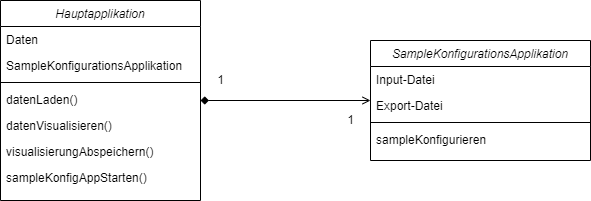
\includegraphics[width=1\linewidth]{konzeptKlassen}
	\caption{Konzept Klassendiagramm}
	\label{fig:konzeptKlassen}
\end{figure}

\section{Ablauf}
Die grundlegenden Benutzung der Applikation soll wie folgt stattfinden. Der Benutzer kann entweder Samples für eine Messung konfigurieren und diese dann im nächsten Schritt innerhalb des Tools visualisieren oder, bei bereits angelegten Samples, diese direkt im Graphen anzeigen. So kann die Erstellung neuer Visualisierungsdaten, aber auch die Wiederverwendbarkeit bereits angelegter Daten gewährleistet werden. Innerhalb eines Ablaufdiagramms lässt sich dies folgendermaßen beschreiben:

\begin{figure}[H]
	\centering
	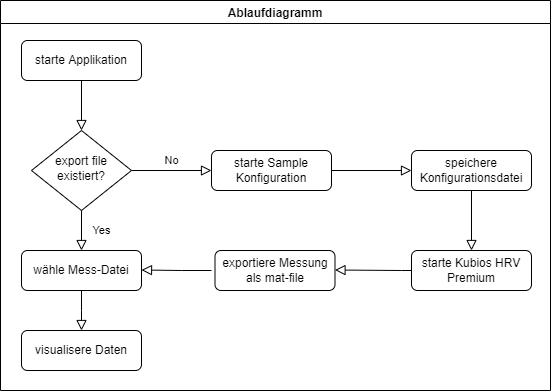
\includegraphics[width=0.8\linewidth]{ablaufKonzept}
	\caption{Ablaufdiagramm des Konzepts}
	\label{fig:ablaufKonzept}
\end{figure}

Für das Erstellen der Samples wurde folgender Ablauf konzipiert. Der Nutzer ruft die Funktion in der Hauptapplikation auf und erhält ein PopUp, in welchem er die Messung und die Parameter zur Konfigurierung einträgt. Im nächsten Schritt wird dies an Kubios HRV Premium weitergeleitet, die Messung  wird dann mittels einer API Schnittstelle oder Ähnlichem in die entsprechenden Samples aufgeteilt und eine Export-Datei im mat-Format erstellt. Danach erfolgt das automatische Einlesen der Datei in die Applikation, der Nutzer kann dann die enstprechend enthaltenen Messparameter visualisieren.

\begin{figure}[H]
	\centering
	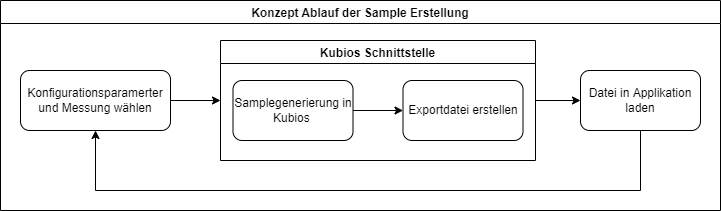
\includegraphics[width=1\linewidth]{konzeptSamples}
	\caption{Konzept Ablauf für das Erstellen der Samples}
	\label{fig:konzeptSamples}
\end{figure}

Für das Visualisieren einzelner Messparametern innerhalb der Applikation wird ein Ablauf wie folgt modelliert. Nach dem das in Kubios erstellte MAT-File in die Applikation geladen wird, kann eine der enthaltenen Parameter in einer Liste ausgewählt werden. Die dazugehörigen Messdaten werden dann im bereits vorhandenen Koordinatensystem angezeigt. Das Visualisieren anderer Parameter erfolgt durch das Auswählen eines anderen Listen-Elements und kann beliebig oft wiederholt werden. 

\begin{figure}[H]
	\centering
	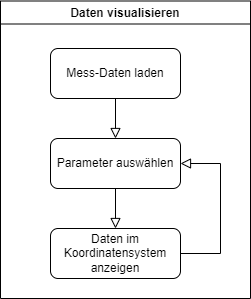
\includegraphics[width=0.35\linewidth]{ablaufVisualisieren}
	\caption{Konzept Ablauf für das Visualisieren von Daten}
	\label{fig:ablaufVisualisieren}
\end{figure}

\section{Applikations-Design}

Das Applikations-Design soll anhand der grundlegenden Regeln des UI Designs implementiert. Dazu gehört in erster Linie der Fokus auf Übersichtlichkeit, Konsistenz der Design-Elemente sowie einfache Bedienbarkeit, welche dem Nutzer im Gedächtnis bleibt und keine große Zeit zur Einarbeitung in Anspruch nimmt. Zudem soll schnell zu erkennen sein, wo welche Funktion aufgerufen und verwendet werden kann. Zuletzt sollen Fehler passend verhindert werden, um das reibungslose Arbeiten mit der Applikation garantieren zu können.

Um diese Grundsätze und Regeln umsezten zu können, soll die Oberfläche keine Verschachtelung enthalten. Alle grundlegenden Funktionen liegen zum Start der Applikation offen und können vor dort aus auch verwendet werden. So soll direkt auf der Startseite der Graph zur Visualisierung sowie die Auswahl der Messparameter zu sehen sein. Kleinere Hilfsfunktionen und Informationen, dazu gehören beispielsweise das Laden von Messdaten oder das Abspeichern der Visualisierung, sollen in eine Menubar am oberen Rand der Applikation integriert werden. Da diese typisch für einen Großteil der Programme ist und so einen Wiedererkennungswert für die Nutzer bietet. 

% Design-Konzept (vielleicht durch Figma Design ersetzen)
\begin{figure}[H]
	\centering
	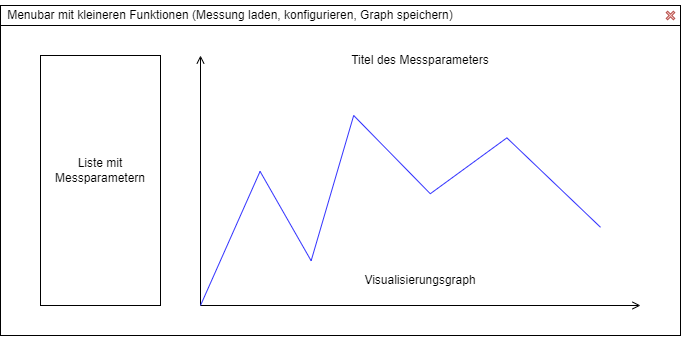
\includegraphics[width=1\linewidth]{designKonzept}
	\caption{Konzept Ablauf für das Design}
	\label{fig:designKonzept}
\end{figure}